

\tikzset{every picture/.style={line width=0.75pt}} %set default line width to 0.75pt        

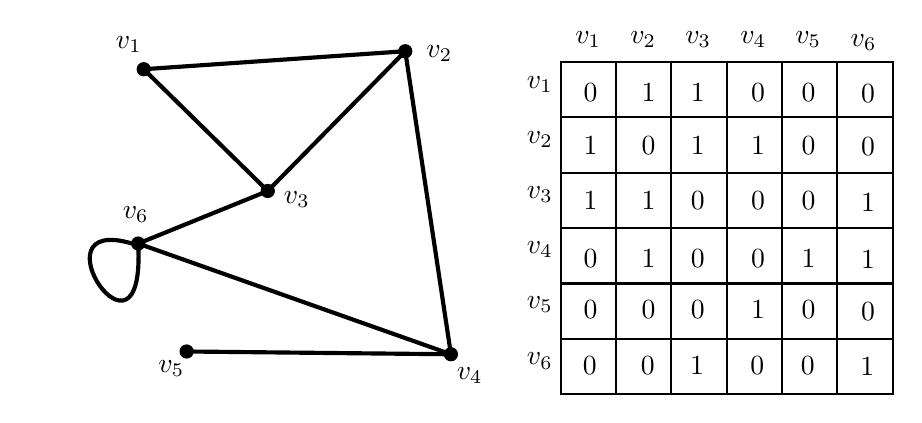
\begin{tikzpicture}[x=0.5pt,y=0.5pt,yscale=-1,xscale=1]
%uncomment if require: \path (0,306); %set diagram left start at 0, and has height of 306

%Shape: Grid [id:dp6535069824522238] 
\draw  [draw opacity=0] (629.64,50.09) -- (389.64,50.09) -- (389.64,290.09) -- (629.64,290.09) -- cycle ; \draw   (589.64,50.09) -- (589.64,290.09)(549.64,50.09) -- (549.64,290.09)(509.64,50.09) -- (509.64,290.09)(469.64,50.09) -- (469.64,290.09)(429.64,50.09) -- (429.64,290.09) ; \draw   (629.64,90.09) -- (389.64,90.09)(629.64,130.09) -- (389.64,130.09)(629.64,170.09) -- (389.64,170.09)(629.64,210.09) -- (389.64,210.09)(629.64,250.09) -- (389.64,250.09) ; \draw   (629.64,50.09) -- (389.64,50.09) -- (389.64,290.09) -- (629.64,290.09) -- cycle ;
%Flowchart: Connector [id:dp13476898875224252] 
\draw  [fill={rgb, 255:red, 0; green, 0; blue, 0 }  ,fill opacity=1 ] (84,55.24) .. controls (84,52.82) and (85.96,50.86) .. (88.38,50.86) .. controls (90.79,50.86) and (92.75,52.82) .. (92.75,55.24) .. controls (92.75,57.65) and (90.79,59.61) .. (88.38,59.61) .. controls (85.96,59.61) and (84,57.65) .. (84,55.24) -- cycle ;
%Flowchart: Connector [id:dp2440554387637338] 
\draw  [fill={rgb, 255:red, 0; green, 0; blue, 0 }  ,fill opacity=1 ] (273,42.24) .. controls (273,39.82) and (274.96,37.86) .. (277.38,37.86) .. controls (279.79,37.86) and (281.75,39.82) .. (281.75,42.24) .. controls (281.75,44.65) and (279.79,46.61) .. (277.38,46.61) .. controls (274.96,46.61) and (273,44.65) .. (273,42.24) -- cycle ;
%Flowchart: Connector [id:dp7387946513087067] 
\draw  [fill={rgb, 255:red, 0; green, 0; blue, 0 }  ,fill opacity=1 ] (306,261.24) .. controls (306,258.82) and (307.96,256.86) .. (310.38,256.86) .. controls (312.79,256.86) and (314.75,258.82) .. (314.75,261.24) .. controls (314.75,263.65) and (312.79,265.61) .. (310.38,265.61) .. controls (307.96,265.61) and (306,263.65) .. (306,261.24) -- cycle ;
%Flowchart: Connector [id:dp4037286088053199] 
\draw  [fill={rgb, 255:red, 0; green, 0; blue, 0 }  ,fill opacity=1 ] (115,259.24) .. controls (115,256.82) and (116.96,254.86) .. (119.38,254.86) .. controls (121.79,254.86) and (123.75,256.82) .. (123.75,259.24) .. controls (123.75,261.65) and (121.79,263.61) .. (119.38,263.61) .. controls (116.96,263.61) and (115,261.65) .. (115,259.24) -- cycle ;
%Straight Lines [id:da5672282422367244] 
\draw [color={rgb, 255:red, 0; green, 0; blue, 0 }  ,draw opacity=1 ][line width=1.5]    (88.38,55.24) -- (277.38,42.24) ;
%Flowchart: Connector [id:dp6922472609995522] 
\draw  [fill={rgb, 255:red, 0; green, 0; blue, 0 }  ,fill opacity=1 ] (173.62,143.24) .. controls (173.62,140.82) and (175.58,138.86) .. (178,138.86) .. controls (180.42,138.86) and (182.38,140.82) .. (182.38,143.24) .. controls (182.38,145.65) and (180.42,147.61) .. (178,147.61) .. controls (175.58,147.61) and (173.62,145.65) .. (173.62,143.24) -- cycle ;
%Straight Lines [id:da758451262727764] 
\draw [color={rgb, 255:red, 0; green, 0; blue, 0 }  ,draw opacity=1 ][line width=1.5]    (178,143.24) -- (277.38,42.24) ;
%Straight Lines [id:da9738303396198353] 
\draw [color={rgb, 255:red, 0; green, 0; blue, 0 }  ,draw opacity=1 ][line width=1.5]    (119.38,259.24) -- (310.38,261.24) ;
%Straight Lines [id:da5325310532938966] 
\draw [color={rgb, 255:red, 0; green, 0; blue, 0 }  ,draw opacity=1 ][line width=1.5]    (310.38,261.24) -- (277.38,42.24) ;
%Straight Lines [id:da34459663888384573] 
\draw [color={rgb, 255:red, 0; green, 0; blue, 0 }  ,draw opacity=1 ][line width=1.5]    (84.38,181.24) -- (178,143.24) ;
%Flowchart: Connector [id:dp2021759841122034] 
\draw  [fill={rgb, 255:red, 0; green, 0; blue, 0 }  ,fill opacity=1 ] (80,181.24) .. controls (80,178.82) and (81.96,176.86) .. (84.38,176.86) .. controls (86.79,176.86) and (88.75,178.82) .. (88.75,181.24) .. controls (88.75,183.65) and (86.79,185.61) .. (84.38,185.61) .. controls (81.96,185.61) and (80,183.65) .. (80,181.24) -- cycle ;
%Curve Lines [id:da22343420131609604] 
\draw [line width=1.5]    (84.38,181.24) .. controls (90,284.24) and (6,159.24) .. (80,181.24) ;
%Straight Lines [id:da9483059964880987] 
\draw [color={rgb, 255:red, 0; green, 0; blue, 0 }  ,draw opacity=1 ][line width=1.5]    (310.38,261.24) -- (84.38,181.24) ;
%Straight Lines [id:da9052215843187655] 
\draw [color={rgb, 255:red, 0; green, 0; blue, 0 }  ,draw opacity=1 ][line width=1.5]    (178,143.24) -- (88.38,55.24) ;

% Text Node
\draw (363,58.09) node [anchor=north west][inner sep=0.75pt]   [align=left] {$\displaystyle v_{1}$};
% Text Node
\draw (363,97.84) node [anchor=north west][inner sep=0.75pt]   [align=left] {$\displaystyle v_{2}$};
% Text Node
\draw (363,137.59) node [anchor=north west][inner sep=0.75pt]   [align=left] {$\displaystyle v_{3}$};
% Text Node
\draw (363,177.34) node [anchor=north west][inner sep=0.75pt]   [align=left] {$\displaystyle v_{4}$};
% Text Node
\draw (363,217.09) node [anchor=north west][inner sep=0.75pt]   [align=left] {$\displaystyle v_{5}$};
% Text Node
\draw (398,25.97) node [anchor=north west][inner sep=0.75pt]   [align=left] {$\displaystyle v_{1}$};
% Text Node
\draw (437.75,25.97) node [anchor=north west][inner sep=0.75pt]   [align=left] {$\displaystyle v_{2}$};
% Text Node
\draw (477.5,25.97) node [anchor=north west][inner sep=0.75pt]   [align=left] {$\displaystyle v_{3}$};
% Text Node
\draw (517.25,25.97) node [anchor=north west][inner sep=0.75pt]   [align=left] {$\displaystyle v_{4}$};
% Text Node
\draw (557,25.97) node [anchor=north west][inner sep=0.75pt]   [align=left] {$\displaystyle v_{5}$};
% Text Node
\draw (481.5,63.09) node [anchor=north west][inner sep=0.75pt]   [align=left] {$\displaystyle 1$};
% Text Node
\draw (481.5,183.09) node [anchor=north west][inner sep=0.75pt]   [align=left] {$\displaystyle 0$};
% Text Node
\draw (481.5,141.59) node [anchor=north west][inner sep=0.75pt]   [align=left] {$\displaystyle 0$};
% Text Node
\draw (525,183.09) node [anchor=north west][inner sep=0.75pt]   [align=left] {$\displaystyle 0$};
% Text Node
\draw (604.5,184.09) node [anchor=north west][inner sep=0.75pt]   [align=left] {$\displaystyle 1$};
% Text Node
\draw (561.5,220.59) node [anchor=north west][inner sep=0.75pt]   [align=left] {$\displaystyle 0$};
% Text Node
\draw (446,63.09) node [anchor=north west][inner sep=0.75pt]   [align=left] {$\displaystyle 1$};
% Text Node
\draw (604.5,102.59) node [anchor=north west][inner sep=0.75pt]   [align=left] {$\displaystyle 0$};
% Text Node
\draw (561.5,101.59) node [anchor=north west][inner sep=0.75pt]   [align=left] {$\displaystyle 0$};
% Text Node
\draw (525,63.09) node [anchor=north west][inner sep=0.75pt]   [align=left] {$\displaystyle 0$};
% Text Node
\draw (561.5,63.09) node [anchor=north west][inner sep=0.75pt]   [align=left] {$\displaystyle 0$};
% Text Node
\draw (604.5,64.09) node [anchor=north west][inner sep=0.75pt]   [align=left] {$\displaystyle 0$};
% Text Node
\draw (446,101.59) node [anchor=north west][inner sep=0.75pt]   [align=left] {$\displaystyle 0$};
% Text Node
\draw (481.5,101.59) node [anchor=north west][inner sep=0.75pt]   [align=left] {$\displaystyle 1$};
% Text Node
\draw (525,101.59) node [anchor=north west][inner sep=0.75pt]   [align=left] {$\displaystyle 1$};
% Text Node
\draw (604.5,142.59) node [anchor=north west][inner sep=0.75pt]   [align=left] {$\displaystyle 1$};
% Text Node
\draw (561.5,141.59) node [anchor=north west][inner sep=0.75pt]   [align=left] {$\displaystyle 0$};
% Text Node
\draw (525,141.59) node [anchor=north west][inner sep=0.75pt]   [align=left] {$\displaystyle 0$};
% Text Node
\draw (525,220.59) node [anchor=north west][inner sep=0.75pt]   [align=left] {$\displaystyle 1$};
% Text Node
\draw (481.5,220.59) node [anchor=north west][inner sep=0.75pt]   [align=left] {$\displaystyle 0$};
% Text Node
\draw (446,220.59) node [anchor=north west][inner sep=0.75pt]   [align=left] {$\displaystyle 0$};
% Text Node
\draw (446,141.59) node [anchor=north west][inner sep=0.75pt]   [align=left] {$\displaystyle 1$};
% Text Node
\draw (446,183.09) node [anchor=north west][inner sep=0.75pt]   [align=left] {$\displaystyle 1$};
% Text Node
\draw (561.5,183.09) node [anchor=north west][inner sep=0.75pt]   [align=left] {$\displaystyle 1$};
% Text Node
\draw (604.5,221.59) node [anchor=north west][inner sep=0.75pt]   [align=left] {$\displaystyle 0$};
% Text Node
\draw (66,29.24) node [anchor=north west][inner sep=0.75pt]   [align=left] {$\displaystyle v_{1}$};
% Text Node
\draw (187.38,141.61) node [anchor=north west][inner sep=0.75pt]   [align=left] {$\displaystyle v_{3}$};
% Text Node
\draw (96.75,263.24) node [anchor=north west][inner sep=0.75pt]   [align=left] {$\displaystyle v_{5}$};
% Text Node
\draw (312.38,268.61) node [anchor=north west][inner sep=0.75pt]   [align=left] {$\displaystyle v_{4}$};
% Text Node
\draw (290.38,35.61) node [anchor=north west][inner sep=0.75pt]   [align=left] {$\displaystyle v_{2}$};
% Text Node
\draw (71,152.24) node [anchor=north west][inner sep=0.75pt]   [align=left] {$\displaystyle v_{6}$};
% Text Node
\draw (363,258.09) node [anchor=north west][inner sep=0.75pt]   [align=left] {$\displaystyle v_{6}$};
% Text Node
\draw (597,27.97) node [anchor=north west][inner sep=0.75pt]   [align=left] {$\displaystyle v_{6}$};
% Text Node
\draw (404,63.09) node [anchor=north west][inner sep=0.75pt]   [align=left] {$\displaystyle 0$};
% Text Node
\draw (404,101.59) node [anchor=north west][inner sep=0.75pt]   [align=left] {$\displaystyle 1$};
% Text Node
\draw (404,220.59) node [anchor=north west][inner sep=0.75pt]   [align=left] {$\displaystyle 0$};
% Text Node
\draw (404,141.59) node [anchor=north west][inner sep=0.75pt]   [align=left] {$\displaystyle 1$};
% Text Node
\draw (404,183.09) node [anchor=north west][inner sep=0.75pt]   [align=left] {$\displaystyle 0$};
% Text Node
\draw (561,260.59) node [anchor=north west][inner sep=0.75pt]   [align=left] {$\displaystyle 0$};
% Text Node
\draw (524.5,260.59) node [anchor=north west][inner sep=0.75pt]   [align=left] {$\displaystyle 0$};
% Text Node
\draw (481,260.59) node [anchor=north west][inner sep=0.75pt]   [align=left] {$\displaystyle 1$};
% Text Node
\draw (445.5,260.59) node [anchor=north west][inner sep=0.75pt]   [align=left] {$\displaystyle 0$};
% Text Node
\draw (604,261.59) node [anchor=north west][inner sep=0.75pt]   [align=left] {$\displaystyle 1$};
% Text Node
\draw (403.5,260.59) node [anchor=north west][inner sep=0.75pt]   [align=left] {$\displaystyle 0$};


\end{tikzpicture}

